\chapter{Dataset and ground truth} %15 pages
\chaptermark{Dataset and ground truth}
\label{chap:gt}
\graphicspath{{./chapters/9-gt/figs/}}
% Abstract-----------------------------------------------------
This chapter\cite{Guerin2013} deals with ...

% -------------------------------------------------------------
\section{Introduction}
\label{sec:gt:intro}

% \begin{itemize}
% 	% \item Contact authors, publishers, they perception of the project
% 	\item Aim to represent the diversity of comics
% 	\item Add comic characters and semantic links
% 	\item Version 2013 and 2014
% \end{itemize}


With the analysis and processing of data comes the need of the output results evaluation.
Traditionally, this evaluation is made by validating the results of an algorithm with a ground truth that represents what an ideal output should be\cite{pascal-voc-2012, smeaton2006evaluation, griffinHolubPerona}.
Ideally, such a ground truth is made publicly available so anyone can challenge his own algorithm to the community \cite{lamiroy:inria-00537035}.
This can be applied to any kind of results from image segmentation to classification or information retrieval.
Being in need of comic books material and an associated ground truth to evaluate our work, we noticed that there is not such dataset publicly available for scientific purpose. 
Therefore, we decided to gather the first publicly available comic books dataset in association with several comic books authors and publishers and to build up the corresponding ground truth according to document analysis and understanding concerns.% which are image segmentation and semantic analysis.

It took almost one year to define which type of comics to use, meet and convince comics authors and publishers, get copyright authorizations for the scientific community, develop a specific annotation tool and finally to hire people to do the ground truth.
Once everything was done, a selection of hundred comic pages were annotated in one day by twenty volunteers affiliated to the L3i lab.
In order to provide a common basis for evaluating research work, the ground truth have been published in 2013~\cite{Guerin2013} and made available to the scientific community via the project website~\footnote{http://ebdtheque.univ-lr.fr}.
It has been enhanced in 2014 by adding semantic information to the already annotated elements.

The content of the dataset, the ground truth construction protocol and its quality assessment are detailed in the next section.


% \section{Structure and indexation}
% \label{sec:gt:structure_indexation}
\section{Dataset description} % (fold)
\label{sec:dataset_description}

% section dataset_description (end)

Scott McCloud defined comics as ``juxtaposed pictorial and other images in deliberate sequence, intended to convey information and/or to produce an aesthetic response in the viewer''~\cite{mccloud1994understanding}.
This definition is intentionally broad enough to encompass the spectrum of the majority of works produced so far.
The dataset composition should reflects this heterogeneity to give everyone the opportunity
to compare its algorithms to a globally representative dataset of the comics world.
We contacted authors with different comic styles and have selected a corpus of one hundred images, representing single or double comics page.

The images were partly processed by the French company A3DNum (\url{http://www.a3dnum.fr}) which was commissioned to digitize 14 albums.
Among all the files, scanned at a resolution of 300 dots per inch and encoded in uncompressed Portable Network Graphic (PNG) format, we used 46 pages to integrate the eBDtheque corpus.
The remaining 54 images were selected from webcomics, public domain comics\footnote{http://digitalcomicmuseum.com} and unpublished artwork with different styles from 72 to 300 dots per inch.
We encoded all the images of the eBDtheque dataset in Joint Photographic Experts Group (JPEG) format with a lossy compression to facilitate file exchange.
%, the non compressed images are available on request.

Hereafter we describe the characteristics of the selected albums and their content.


\paragraph{Albums} % (fold)
 \label{par:albums}
 published between 1905 and 2012.
 29 pages were published before 1953 and 71 after 2000.
 Quality paper, colour saturation and textures related to printing technique changes can vary a lot from one page to another.
 The artworks are mainly from France (81\%), United States (13\%) and Japan (6\%).
 Their styles varies from classical Franco-Belgium ``bandes dessinées'' to Japanese manga through webcomic and American comics.

 % paragraph albums (end)

\paragraph{Pages} % (fold)
\label{par:pages}
 themselves have very diverse characteristics.
Among all, 72 are printed in colours and according to the authors and periods, there are a majority of the tint areas, watercolours and hand-coloured areas.
Among the remaining 28, 16 have are greyscale and 12 are simply black and white.
One album has two versions of each page, one in colour and the other one in black and white.
We have integrated an examples of each of them in order to allow performance comparison of algorithms on the same graphic style by using colour information or not.
Five of the 100 images are double page, others are single page and 20\% are not A4 format.
%We therefore, strictly speaking, 105 and 100 pages not in our database, each with a distinct structure
% paragraph pages (end)

\paragraph{Panels} % (fold)
\label{par:panels}
 contained in the pages are of various shapes.
Although most of them are bounded by a black line, a significant proportion has at least one part of the panel which is indistinguishable from the background of the page (frame less panel).
Two pages consist only of frame less panels, the visual delimitation uses background contrast difference between the panel and image.
Nine images contain overlapping panels, twelve contain only panels without border and several has panels connected by an straddle object.

% paragraph panels (end)

\paragraph{Balloons} % (fold)
\label{par:balloons}
 also contain a great diversity.
Some of them are completely surrounded by a black stroke, some partially and others not at all.
They have a bright background with a rectangular, oval or non geometric shape with ``smooth'', ``wavy'' or ``spiky'' contour in general.
Most of them has a tail pointing towards the speaker, but some do not.
There is text without any surrounding balloons on 33 images of the corpus.
% and 8 of them simply contain no bubble.

% paragraph balloons (end)

\paragraph{Text} % (fold)
\label{par:text}
 is either typewritten (61\% of the image) or handwritten, mainly upper-case.
The text lines contains 12 elements in average (see figure~\ref{fig:gt:textline_lenth_distribution}) and there are more than hundred text lines that are composed by only one letter which are punctuation or single letter words such as ``I'' or ``A''.

Most pages are from French artworks, where the text is written in French.
Only 13 pages contain English text and 6 images are in Japanese.
Onomatopoeia appears in 18 pages.

    %%%%%%%%%%%%%%%%%%%%%%%%%%%%%%%%%%%%%%%%%%%%%%%%%%%%%%%%
    \begin{figure}[ht]%trim=l b r t  width=0.5\textwidth,  
      \centering
      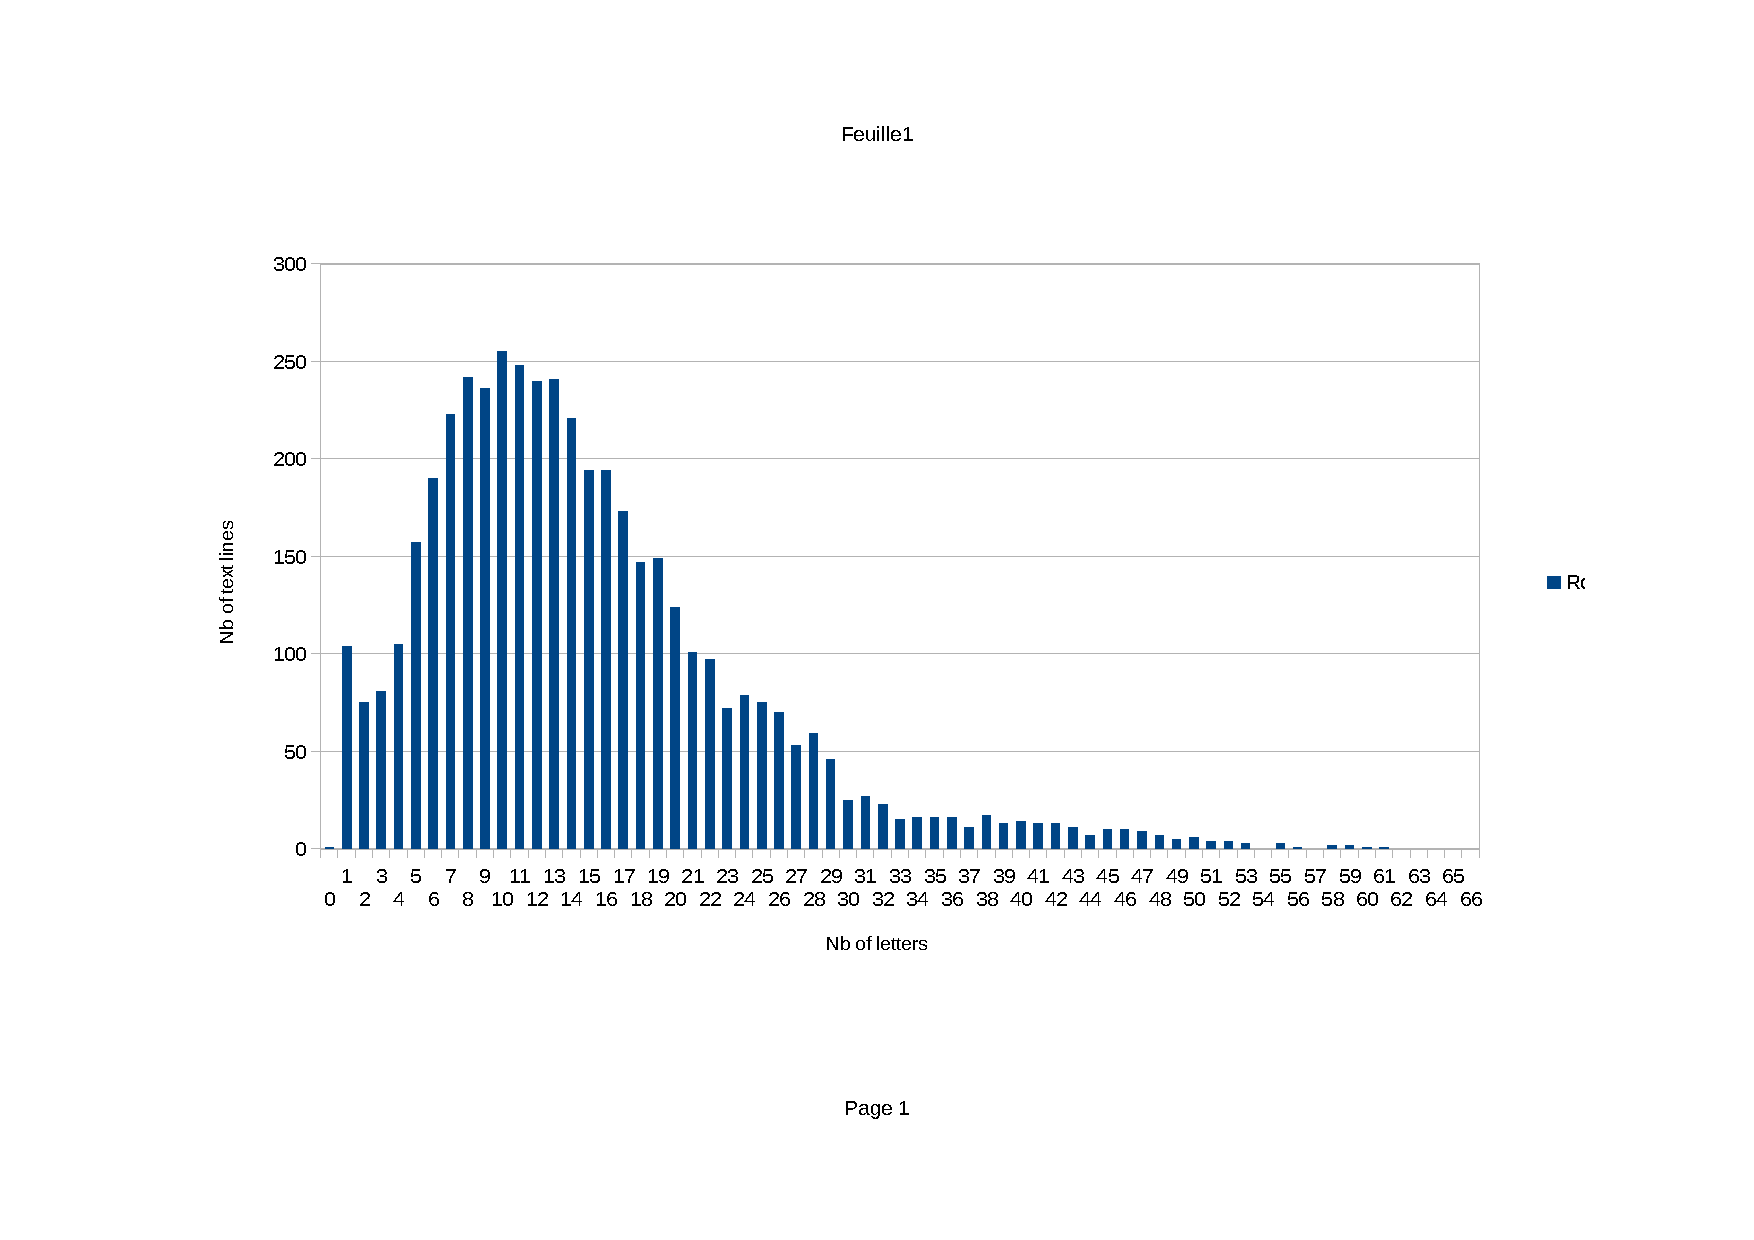
\includegraphics[trim= 100px 130px 120px 120px, clip, width=0.65\textwidth]{number_of_letter_per_textline.pdf}
      \caption{Distribution of the number of elements per text lines.
      }
      \label{fig:gt:textline_lenth_distribution}
    \end{figure}  
    %%%%%%%%%%%%%%%%%%%%%%%%%%%%%%%%%%%%%%%%%%%%%%%%%%%%%%%%

% paragraph text (end)

\paragraph{Comic characters} % (fold)
\label{par:comic_characters}
or protagonist are specific to each album.
They all have eye, harm and leg but at least 50\% are not humanoid, depending on the interpretation.
% paragraph comic_characters (end)


\section{Ground truth construction} % (fold)
\label{sec:ground_truth_construction}
In order to cover a wide range of possible research matters, it has been decided to extract three different type of objects from the corpus: text lines, balloons and panels.
We decided to do this first ground truth by drawing horizontal bounding boxes as close as possible from the feature and including all its pixels.
% in order to proceed a maximum of pages in the allowed time. 
We chose this level of granularity in order to limit the subjectiveness of the person making the annotation.

The comics art is extremely heterogeneous and our dataset voluntarily integrates albums that can be classified as
unconventional.
This leaves room for interpretation on the form which increase annotation variations by different people and decrease the uniformity of the ground truth.
This precision level is used in several, widely used datasets~\cite{pascal-voc-2012, yao2007introduction}.
%{\color{blue}This groundtruthing level is also used for well known dataset widely used~\cite{pascal-voc-2012, yao2007introduction}.}
Hereafter we define each element to annotate and the protocol to follow.
% follows specific guidelines according to the rules below:

\subsection{Visual annotation} % (fold)
\label{sub:visual_annotation}

% subsection visual_annotation (end)
\paragraph{Panels} % (fold)
\label{par:panels}
are defined as an image area, generally rectangular, representing a single scene in the story. 
There is always at least one panel per page, the entire page region can be used as panel if necessary.
When a panel has a black border, the bounding box is placed as close as possible to its frame.
Sometimes, images have not been scanned perfectly horizontally, it is then impossible to have an horizontal bounding box sticking exactly to the border.
When the panel border is partially absent or suggested by the neighbourhood, the bounding box just defines the content of the panel.
In all cases, the other elements (balloon, text, drawings) extending from the frame are truncated, see figure~\ref{fig:gt:segPanel}.

%%%%%%%%%%%%%%%%%%%%%%%%%%%%%%%%%%%%%%%%%%%%%%%%%%%%%%%%%
\begin{figure}[h!]
\begin{center}
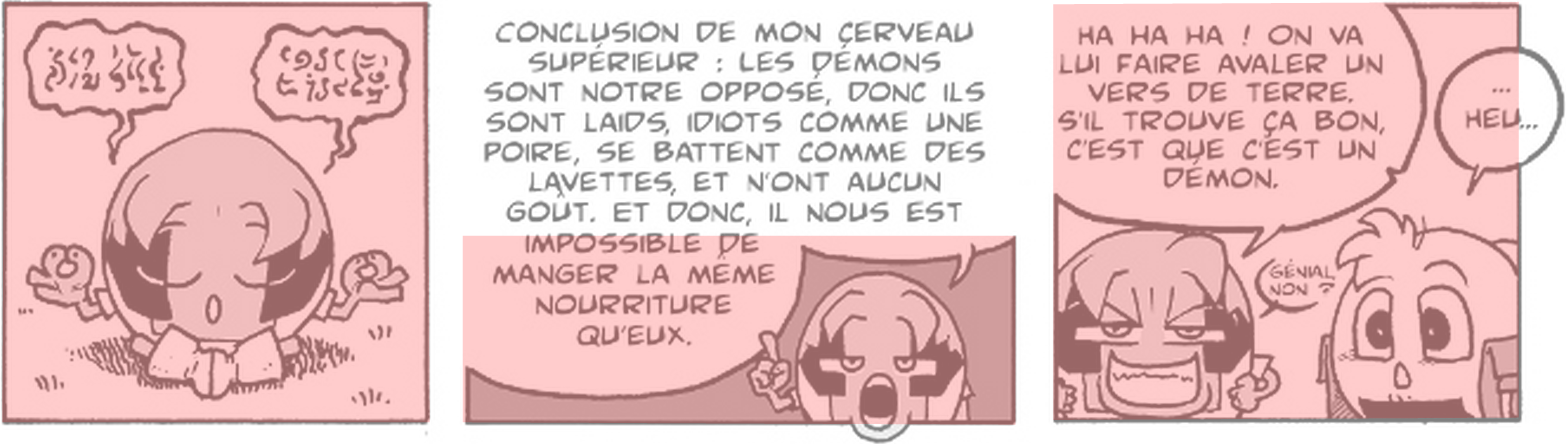
\includegraphics[width=0.8\textwidth]{segPanel.png}
\caption[Panel annotation]{Example of three panel annotations. The bounding box (transparent red) is defined without taking into account of non panel elements in all cases.}
\label{fig:gt:segPanel}
\end{center}
\end{figure}
%%%%%%%%%%%%%%%%%%%%%%%%%%%%%%%%%%%%%%%%%%%%%%%%%%%%%%%%%

%They can be frame-less, in that case the bounding box will be set according to the contained drawings, see Fig. \ref{fig:segmentation}c. %, ignoring text and overlapping features.
%In both cases, text and overlapping features are ignored.
%There is necessarily at least one panel in a page. 
% paragraph panels (end)

% The panel reading order is also annotated in a metadata called \texttt{rank}, it is in integer  between $1$ and $n$ which is increased incrementally from the first to the last panel $n$ in an image.%, le premier de la séquence prenant la valeur $1$ et le dernier la valeur $n$ pour une page contenant $n$ cases.

\paragraph{Balloons} % (fold)
\label{par:balloons}
We define a balloon (phylactery) as the region of an image including one or several lines of text, graphically defined by an identifiable physical boundary or suggested by the presence of an arrow pointing to the speaker (the tail).
Although rare, empty balloons (not containing lines of text) are also annotated if they are clearly identifiable by their shape or
the tail representation.
Pixel level annotation follows the contour of the balloon (see figure~\ref{fig:gt:segBalloons}c), while bounding box annotation does not consider the contour of phylactery and truncates the tail.
Sometimes it crosses the entire panel and generates an unrepresentative position of the desired balloon (see figure~\ref{fig:gt:segBalloons}a).
When the balloon is not closed (e.g. open contour) the annotated contour has to stick as close as possible to the contained text (see figure~\ref{fig:gt:segBalloons}b).
Note, the first version of the ground truth have been defined at bounding box level ignoring the tail and the second version at pixel level following the contour variations and the tail region.


\begin{figure}[h!]
\begin{center}
\begin{tabular}{ccc}
a) 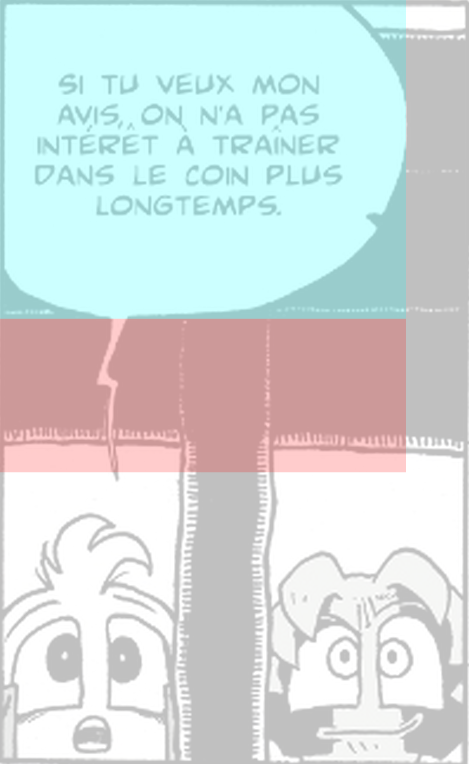
\includegraphics[width=80px]{segBalloon1.png} 
& 
b) 
\includegraphics[width=80px]{segBalloon2.png}
&
c) 
\includegraphics[width=80px]{segBalloon3.png}
\end{tabular}
\caption[Speech balloon contour annotation]{Example of balloon clipping: a) using bounding box excluding the tail, b) bounding box of non closed balloon, c) pixel level contour annotation.} 
\label{fig:gt:segBalloons}
\end{center}
\end{figure}

% paragraph balloons (end)

\paragraph{Text lines} % (fold)
\label{par:text_lines}
The text lines are defined as a sequence of text characters aligned in the same direction (see figure~\ref{fig:gt:segLines}a).
This definition encompasses both speech texts and narrative text, often located inside balloon, onomatopoeia (graphic sound) that are written or drawn directly in the panel without particular container.
%The text of the latter, although they are occasionally parallel to the edges of the box is still clipped by a horizontal bounding box for consistency across the ground truth.
Comics are static graphics, the expression of emotions of a comic character is the joint action of drawing and text, sometimes in the form of a single punctuation symbol.
For instance, an exclamation mark for surprise or a question mark for a misunderstanding.
These isolated symbols convey information and are segmented as text line as well (see figure~\ref{fig:gt:segLines}b).
Similarly, we have chosen to include in this category the illustrative text, such as a road sign or storefront (see figure~\ref{fig:gt:segLines}c).
Although at the boundary between text and graphic, these elements are still invariably read by the reader and their annotation is potentially interesting for multiple purposes, including story and scene analysis.


\begin{figure}[h!]
\begin{center}
\begin{tabular}{ccc}
a) 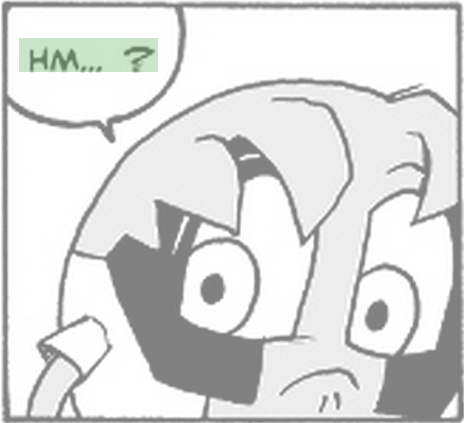
\includegraphics[width=80px]{segLine1.png} 
& 
b) 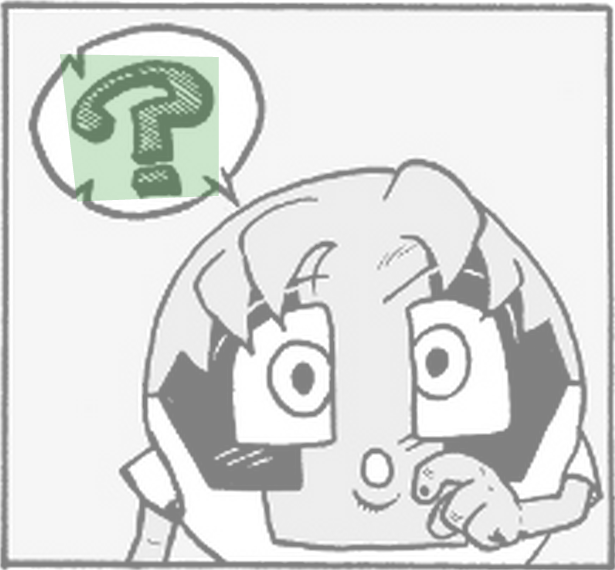
\includegraphics[width=80px]{segLine2.png}
&
c) 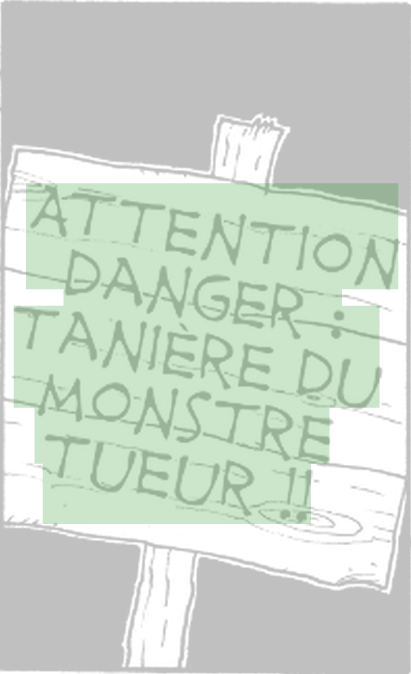
\includegraphics[width=80px]{segLine3.png}
\end{tabular}
\caption[Text line location annotation]{Different examples of text line position annotation: a) a classical text line in a speech balloon, b) a unique symbol, c) illustrative text, non horizontal.} 
\label{fig:segLines}
\end{center}
\end{figure}
% paragraph text_lines (end)

\paragraph{Comic characters} % (fold)
\label{par:comic_characters}


% paragraph comic_characters (end)


% section ground_truth_construction (end)

\subsection{Semantic annotation} % (fold)
\label{sub:semantic_annotation}
Once segmented, each object is annotated with a set of predefined metadata as follows. 

\subsubsection{Panels} 
Each panel is annotated with a \texttt{{rank}} metadata which stand for its  position in the reading sequence. 
The first panel to be read on a given page has its rank property set to 1, while the last one's is set to \textit{n}, with \textit{n} the number of panels in the page.

\subsubsection{Balloons}
Balloons are also annotated with a \texttt{{rank}} property. 
However, as balloons are not explicitly bounded to any panel, their rank is set according to the page as a whole. 
For a page containing {\it m} balloons, the first balloon's rank will be 1 and the last will be {\it m}.
Moreover, two additional metadata are given. 
First, the \texttt{{shape}} is indicated, picking a value from the enumeration \{\texttt{cloud, oval, peak, rectangle, suggested}\} as pictured in Fig. \ref{fig:balloons_shape}.
Finally, the pointing direction of a  balloon's tail is given through the \texttt{{queueDirection}} property. 
The possible values are the eight cardinal directions plus a ninth additional value for the lack of a tail: \{\texttt{N, NE, E, SE, S, SW, W, NW, none}\}.

\subsubsection{Text lines}
Each text line is associated with its transcription in capital letters.

\subsubsection{Pages}\label{sec:pages}
Each page has been annotated with bibliographical information, so that anyone using this database can find the appropriate comic books. 
Among the first ones comes the page number (\texttt{{pageNumber}}) the comic book title, from which the page has been picked up, and its release date (\texttt{{albumTitle, releaseDate}}), the series it belongs to (\texttt{{collectionTitle}}), the authors and editor names (\texttt{{writerName, drawerName, editorName}}) and, finally, the website and/or ISBN (\texttt{{website, ISBN}}). The album title is not mandatory for webcomics.
Structural information about the page content has been added as well, such as resolution (\texttt{{resolution}}), reading direction (\texttt{{readingDirection}}), main language of the written text (\texttt{{language}}) and single or double page image (\texttt{{doublePage}}).

%%%%%%%%%%%%%%%%%%%%%%%%%%%%%%%%%%%%%%%%%%%
% \begin{figure}
% \begin{center}
% \includegraphics[width=0.45\textwidth]{balloons_shape3.png}
% \caption{Different speech balloon shapes. Top-down, from left to right: cloud, peak, suggested, rectangular and oval.}
% \label{fig:balloons_shape}
% \end{center}
% \end{figure}
%%%%%%%%%%%%%%%%%%%%%%%%%%%%%%%%%%%%%%%%%%%

The combination of visual and semantic annotation provides the advantage to make this ground truth relevant for document analysis and semantic evaluation which are both part of the comics understanding process.
% subsection semantic_annotation (end)

\subsection{File structure} % (fold)
\label{sub:file_structure}
As we wanted to keep the database file system simple and easy to share, semantic and visual annotations on a given page are gathered in a single SVG (Scalable Vector Graphics) file. 
Besides being royalty-free and actively maintained by a W3C working group, the SVG format fulfils two essential needs for this database.

First, in association with a recent Internet browser or your favorite image viewer, it provides a simple, fast and elegant way to display the visual segmentation of any desired object over a comic book page. 
Different kind of objects (e.g. panels, balloons) can be displayed in different ways according to CSS (Cascading Style Sheets) properties defined for each of them, see Fig. \ref{fig:css}. 
Each layer can be displayed or not in order to enhance the clearness of the annotations when browsing the database.
Secondly, SVG being a XLM-based language, it makes the integration of semantic annotation very easy via the use of the predefined \texttt{metadata} element.

One ground truth file contains the complete description of one comics image. 
There is no hierarchical link between pages from a same comic book. 
Following the basic XML and encoding information, a SVG file starts with a root \texttt{<svg>} element containing the title of the document, \texttt{<title>}, and four \texttt{<svg>} children with different class attributes.
%A SVG file begins with information about the XML version and encoding system and then a root \texttt{<svg>} element containing the title of the document \texttt{<title>} and four others \texttt{<svg>} elements with different class attributes. % that describe the page, the panels, the text lines and the text areas the entire set of annotations for the attached page.
The annotations are the same for all the \texttt{<svg>} nodes, each of them describing one kind of element (e.g. panel, balloon) according to its {\tt class} attribute. 
The first \texttt{<svg>} element, \texttt{<svg class=``Page''>}, has two children.
The first one is \texttt{<image>} and contains a link to the corresponding image file and the size it has to be displayed.
The next child is a \texttt{<metadata>} element containing the bibliographical information described in \ref{sec:pages}.
The three following \texttt{<svg>} siblings, \texttt{<svg class=``Panel''>}, \texttt{<svg class=``Balloon''>} and \texttt{<svg class=``Line''>} respectively contain the annotations on panels, balloons and text lines. 
They all contain SVG \texttt{<polygon>} elements with a list of five points in a \texttt{point} attribute that define the position of the bounding box's corners. %four corners position coordinates of a bounding box. 
Note that the fifth point equal the first one to ``close'' the polygon according to the SVG format. 
Those points are used by the viewer to draw polygons over the page. 
Each \texttt{<polygon>} has a \texttt{<metadata>} child to store information on the corresponding polygon, according to the attributes list described in \ref{sec:semanticAnnotation}.

%{\bf Add SVG code figure here?} Arnaud suggested it too but, we don't have room and it will be ugly...

%
%\begin{lstlisting}
%<svg>
%</svg>
%\end{lstlisting}

%{\color{red}short file as an illustration?}

% \begin{figure}
% \begin{center}
% \begin{tabular}{ccc}
% \includegraphics[width=0.14\textwidth]{fig/bbg_panel2.png} & 
% \includegraphics[width=0.14\textwidth]{fig/bbg_balloon2.png} &
% \includegraphics[width=0.14\textwidth]{fig/bbg_textlines2.png}
% %\includegraphics[width=0.20\textwidth]{fig/bbg_all.png} &
% \end{tabular}
% \caption{Left-to-right: segmentation of a panel, a speech balloon and text lines. Credits: \cite{Bubble09}}
% \label{fig:css}
% \end{center}
% \end{figure}
% subsection file_structure (end)

\begin{itemize}
	\item Comic Book Markup Language \url{http://digitalhumanities.org/dhq/vol/6/1/000117/000117.html}
\end{itemize}

\section{Ground truth quality assessment}
\label{sec:gt:ground_truth_quality_assessment}


% \section{Discussions}
% \label{sec:gt:siscussions}


\section{Conclusions}
\label{sec:ncrag:concl}
Published in ICDAR'13